% Options for packages loaded elsewhere
\PassOptionsToPackage{unicode}{hyperref}
\PassOptionsToPackage{hyphens}{url}
%
\documentclass[
]{article}
\usepackage{amsmath,amssymb}
\usepackage{lmodern}
\usepackage{iftex}
\ifPDFTeX
  \usepackage[T1]{fontenc}
  \usepackage[utf8]{inputenc}
  \usepackage{textcomp} % provide euro and other symbols
\else % if luatex or xetex
  \usepackage{unicode-math}
  \defaultfontfeatures{Scale=MatchLowercase}
  \defaultfontfeatures[\rmfamily]{Ligatures=TeX,Scale=1}
\fi
% Use upquote if available, for straight quotes in verbatim environments
\IfFileExists{upquote.sty}{\usepackage{upquote}}{}
\IfFileExists{microtype.sty}{% use microtype if available
  \usepackage[]{microtype}
  \UseMicrotypeSet[protrusion]{basicmath} % disable protrusion for tt fonts
}{}
\makeatletter
\@ifundefined{KOMAClassName}{% if non-KOMA class
  \IfFileExists{parskip.sty}{%
    \usepackage{parskip}
  }{% else
    \setlength{\parindent}{0pt}
    \setlength{\parskip}{6pt plus 2pt minus 1pt}}
}{% if KOMA class
  \KOMAoptions{parskip=half}}
\makeatother
\usepackage{xcolor}
\IfFileExists{xurl.sty}{\usepackage{xurl}}{} % add URL line breaks if available
\IfFileExists{bookmark.sty}{\usepackage{bookmark}}{\usepackage{hyperref}}
\hypersetup{
  hidelinks,
  pdfcreator={LaTeX via pandoc}}
\urlstyle{same} % disable monospaced font for URLs
\usepackage{graphicx}
\makeatletter
\def\maxwidth{\ifdim\Gin@nat@width>\linewidth\linewidth\else\Gin@nat@width\fi}
\def\maxheight{\ifdim\Gin@nat@height>\textheight\textheight\else\Gin@nat@height\fi}
\makeatother
% Scale images if necessary, so that they will not overflow the page
% margins by default, and it is still possible to overwrite the defaults
% using explicit options in \includegraphics[width, height, ...]{}
\setkeys{Gin}{width=\maxwidth,height=\maxheight,keepaspectratio}
% Set default figure placement to htbp
\makeatletter
\def\fps@figure{htbp}
\makeatother
\setlength{\emergencystretch}{3em} % prevent overfull lines
\providecommand{\tightlist}{%
  \setlength{\itemsep}{0pt}\setlength{\parskip}{0pt}}
\setcounter{secnumdepth}{-\maxdimen} % remove section numbering
\ifLuaTeX
  \usepackage{selnolig}  % disable illegal ligatures
\fi

\author{}
\date{}

\begin{document}

\hypertarget{stage-logboek-week-5-21032022---25032022}{%
\section{Stage logboek: Week 5 (21/03/2022 -
25/03/2022)}\label{stage-logboek-week-5-21032022---25032022}}

\hypertarget{maandag-21032022}{%
\subsection{Maandag 21/03/2022}\label{maandag-21032022}}

werkuren: \emph{08:00-16:00}

Verder gewerkt aan de denkoefening om high availability te implementeren
bij databanken. Tom heeft voor mij een aantal virtuele machines laten
maken zodat ik hierop kan testen.

Stageverslag verder aangevuld.

\hypertarget{dinsdag-22032022}{%
\subsection{Dinsdag 22/03/2022}\label{dinsdag-22032022}}

Geen stage.\\
Jobevent van HoGent

\hypertarget{woensdag-23032022}{%
\subsection{Woensdag 23/03/2022}\label{woensdag-23032022}}

werkuren: \emph{8:00 - 16:00}

Verder gewerkt aan de denkoefening om high availability te implementeren
bij databanken: Testopstelling gemaakt.

\begin{itemize}
\tightlist
\item
  databank master
\item
  databank slave
\item
  reverse proxy
\end{itemize}

\begin{figure}
\centering
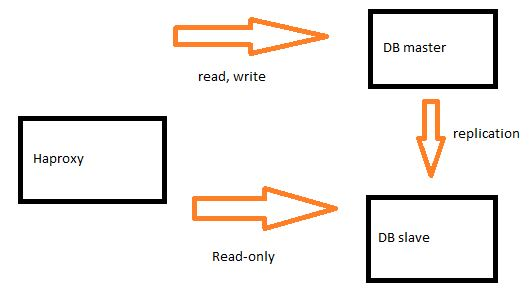
\includegraphics{../notes/img/networkdiagram_db_replication.JPG}
\caption{netwerk diagram}
\end{figure}

Er is nog uitbreiding mogelijk: Hoe van replica een master maken?

\hypertarget{donderdag-24032022}{%
\subsection{Donderdag 24/03/2022}\label{donderdag-24032022}}

Fysiek in Peutie

werkuren: \emph{8:00 - 16:00}

Introductie van \emph{mssql}\\
Onderzoeksopdracht besproken. ik zal hierover nog een document
ontvangen.\\
Tom heeft mij een rondleiding gegeven in de serverroom van in Peutie.

In de namiddag was er een drink binnen defensie waar de kolonel een
toespraak heeft gehouden. Het was tof om deze bij te wonen.

\end{document}
